\chapter{Stand der Forschung und technische Grundlagen}

Dieses Kapitel dient dem Leser als Überblick über die für diese Arbeit relevanten Forschungsgebiete und ihre Methoden. Außerdem werden zusätzlich technische Grundlagen erläutert. Zunächst erfolgt eine Einführung in das Forschungsfeld der Kontinuumsrobotik. Insbesondere richtet sich der Fokus auf etablierte Modelle zur kinematischen Beschreibung kontinuierlicher Manipulatoren. Eine Formulierung der Vorwärtskinematik für den in dieser Arbeit behandelten kontinuierlichen Manipulator findet statt. Bereits bestehende Möglichkeiten, die inverse Kinematik zu beschreiben, werden diskutiert.
%In diesem Zusammenhang findet ein Vergleich unterschiedlicher Darstellungen von Orientierungen eines Körpers im kartesischen Raum statt. 
Anschließend wird das \textit{Reinforcement Learning} (RL) im Kontext des \textit{Machine Learning} (ML) eingeordnet. Wesentliche Bestandteile des RL werden erläutert. Insbesondere wird die Approximation von Funktionen mittels \textit{Artificial Neural Nets} (ANN) beschrieben. Zuletzt erfolgt eine Abgrenzung der bestehenden, inversen Kinematikmodelle zu dem in dieser Arbeit herausgearbeiteten Vorgehen. 

%Wesentliche Bestandteile des RL bilden der episodische \textit{Markov Decision Process} (MDP) sowie die allgemeine Zielsetzung den zukünftig, erwarteten \textit{reward} zu maximieren.

%Zuletzt wird der in dieser Arbeit verwendete Ansatz zur Lösung der inversen Kinematik eines aus zwei Segmenten bestehenden seilzugaktuierten Kontinuumsroboters vorgestellt und mit bereits existierenden Lösungen verglichen.

\section{Kontinuumsrobotik}
\label{sec:kontinuumsrobotik}

Der Urpsprung der Kontinuumsrobotik lässt sich auf die Sechzigerjahre des 20. Jahrhunderts zurückführen. Im Jahr 1968 ließen sich Anderson und Horn den \textit{Tensor arm manipulator}\footnote{https://patents.google.com/patent/US3497083 (aufgerufen am 25.07.2018)}, welcher mithilfe von insgesamt 40 Seilzügen und zehn miteinander verbundenen Platten aktuiert wird, patentieren. Der \textit{Tensor arm manipulator} gilt als einer der ersten Kontinuumsroboter~\cite{Wal13}. Oftmals dienen Vorbilder aus dem Tierreich als Inspiration für die Gestaltung kontunierlicher Manipulatoren. Elefantenrüssel, Tentakel von Kraken und Schlangen bilden prominente Beispiele, welche gemeinsam mit ihren nachgebildeten Robotern in Bild~\ref{fig:tiereUndRoboter} illustriert sind. Bei den Nachbildungen geht es nicht vorrangig darum, das Vorbild aus der Natur möglichst genau zu kopieren. Stattdessen versucht man, die herausragenden Eigenschaften von den dargestellten und weiteren Tieren in der Domäne der Robotik umzusetzen und sich zunutze zu machen. Die vermutlich bedeutendste Eigenschaft kontinuierlicher Manipulatoren ist ihre Flexibilität und Nachgiebigkeit, welche es ihnen ermöglicht, sich kontinuierlich zu krümmen. Dieses Merkmal ist ein wesentlicher Bestandteil verschiedener Definitionen von Kontinuumsrobotern. Im Jahr 1999 definieren Robinson und Davies zunächst~\cite{RD99}:
%
\begin{figure}[t]
% alle bilder sind ausgeschnitten mit 640 x 427 pixels
\centering
\subcaptionbox{Elefantenrüssel\protect\footnotemark}%
[.32\linewidth]{\includegraphics[width=.32\linewidth]{bilder/standdertechnik/elephant_trunk_crop.jpg}}
\subcaptionbox{Oktopus\protect\footnotemark}%
[.32\linewidth]{\includegraphics[width=.32\linewidth]{bilder/standdertechnik/octopus.jpg}}
\subcaptionbox{Schlange\protect\footnotemark}
[.32\linewidth]{\includegraphics[width=.32\linewidth]{bilder/standdertechnik/snake.jpg}}
\medskip
\subcaptionbox{Elefantenrüssel-manipulator \cite{WH99}}%
[.32\linewidth]{\includegraphics[width=.32\linewidth]{bilder/standdertechnik/elephant_trunk_robot2_crop.png}}
\subcaptionbox{OctArm \cite{COW08}\label{sf:octarmGrap}}%
[.32\linewidth]{\includegraphics[width=.32\linewidth]{bilder/standdertechnik/octarm2_crop.png}}
\subcaptionbox{ACM-R3 \cite{HY09}}
[.32\linewidth]{\includegraphics[width=.32\linewidth]{bilder/standdertechnik/acm_r3_crop.png}}
\caption[Vorbilder für Kontinuumsroboter aus dem Tierreich und an sie angelehnte Nachbildungen]{Vorbilder für Kontinuumsroboter aus dem Tierreich und an sie angelehnte Nachbildungen}
\label{fig:tiereUndRoboter}
\end{figure}

\begin{quotation}
\textit{Continuum robots do not contain rigid links and identifiable rotational joints. Instead the structures bend continuously along their length via elastic deformation and produce motion through the generation of smooth curves, similar to tentacles or tongues of the animal kingdom.}
\end{quotation}

Auch die Definition von Walker im Jahr 2013 greift diesen Punkt auf und grenzt kontinuierliche Manipulatoren zusätzlich von seriellen Robotern ab~\cite{Wal13}:

\begin{quotation}
\textit{These robots, termed continuum robots, can be viewed as being ``invertebrate`` robots, as compared with ``vertebrate`` design of conventional rigid-link robots. Continuum robots can bend (and often extend/contract and sometimes twist) at any point along their structure.}
\end{quotation}

%%%%%%%%%%%%%%%%%%%%%%%%%%%%%%%%%%%%%%%%%%%%%%%%%%%%%%%%%%%%%%%%%%%%
\footnotetext[2]{https://commons.wikimedia.org/wiki/File:Elephant\_trunk\_(1).jpg (aufgerufen am 26.07.2018)}
\footnotetext[3]{https://commons.wikimedia.org/wiki/File:Pinnoctopus\_cordiformis.jpg (aufgerufen am 26.07.2018)}
\footnotetext[4]{https://commons.wikimedia.org/wiki/File:Chrysopelea\_taprobanica.jpg (aufgerufen am 26.07.2018)}
%%%%%%%%%%%%%%%%%%%%%%%%%%%%%%%%%%%%%%%%%%%%%%%%%%%%%%%%%%%%%%%%%%%%%

Eine aktuellere Definition von Burgner und Rucker aus dem Jahr 2015 verallgemeinert den Begriff des Kontinuumsroboters wie folgt~\cite{BRC15}. 

\begin{quotation}
\textit{A continuum robot is an actuatable structure whose constitutive material forms curves with continuous tangent vectors.}
\end{quotation}

Die oben aufgeführten Definitionen grenzen direkt und indirekt Kontinuumsroboter von den in der Industrie etablierten seriellen Roboter mit einer rigiden Struktur ab. Anstelle von mehreren, steifen, über Gelenke miteinander verbundene Glieder besitzen Kontinuumsroboter oft ein sich kontinuierlich biegsames Rückgrat. Eine daraus abgeleitete und erwünschte Eigentschaft kontinuierlicher Manipulatoren ist, in schwer zugänglichen Umgebungen navigieren und manövrieren zu können ist . Die inhärente Nachgiebigkeit unterstützt die Fähigkeit, sich in gewundenen Hohlräumen der äußeren Struktur anzupassen. Kontinuumsroboter unterscheiden sich zusätzlich von seriellen Robotern in der Art und Weise, wie sie ihre Umwelt manipulieren können. Während serielle Roboter mittels speziell angefertigter Endeffektoren Gegenstände greifen und bewegen, sollen kontinuierliche Roboter ähnlich wie Elefantenrüssel oder Tentakel zusätzlich in der Lage sein, Gegenstände mit ihrer gesamten Struktur zu umschließen~\cite{Moc01}, siehe Bild~\ref{fig:tiereUndRoboter}\,(e).

Walker unterteilt in~\cite{Wal13} kontinuierliche Manipulatoren in drei durch ihr Design und ihre Aktuierung bestimmte Gruppen. Die erste Gruppe bilden \textit{seilzugaktuierte Kontinuumsroboter}, welche durch Verkürzen und Verlängern von Seilzügen, die entlang des kontinuierlichen Manipulators angebracht sind, die Form des Roboters bestimmen. 

Zur zweiten Gruppe gehören \textit{tubuläre Kontinuumsroboter}. Es werden mehrere konzentrisch ineinander verbaute Röhrchen bewegt und rotiert, um Translationen und Torsionen des Endeffektors zu erzeugen. Mittels einer zusätzlichen Vorbiegung der Röhrchen ist es möglich, eine kontinuierliche Krümmung zu erzeugen. 
Die ersten beiden Gruppen werden extrinisische Manipulatoren gennant, da die Aktorik außerhalb von dem eigentlichen Manipulator angebracht ist. Eine Folge der extrinsischen Aktuierung ist die Realisierung kompakter und filligraner Designs des eigentlichen Manipulators. 

Die dritte Gruppe gehört zu den intrinsischen Manipulatoren und Walker nennt diese \textit{lokal aktuierte Rückgratdesigns}. Hier sind die Aktoren Teil der eigentlichen Rückgratstruktur und somit direkt an der Formgebung beteiligt. Sogenannte pneumatisch bewegte \textit{McKibben-Muskeln} können hier als Aktoren dienen. Jeweils ein Beispiel der oben angegebenen Gruppen ist in Bild~\ref{fig:dreiKontinuumsRoboter} zu sehen. \newline

Im Rahmen dieser Arbeit wird ein seilzugaktuierter Kontinuumsroboter bestehend aus zwei Segmenten kinematisch modelliert, da dieser den kontinuierlichen, kinematischen Ketten im Forschungsprojekt \textit{Parallel-kontinuierliche Manipulatoren} des \textit{LKR} und des \textit{imes} ähnelt. An jedem Segment enden jeweils drei Seilzüge, wodurch der Roboter insgesamt sechs Freiheitsgrade aufweist. Grundsätzliche Eigenschaften der Kinematik sind Gegenstand des nächsten Abschnitts.

\begin{figure}[t!]
% all pictures are resized to 640 x 480 pixels
\centering
\subcaptionbox{Seilzugaktuierter \\Manipulator~\cite{NB16}}[.32\linewidth]
{\includegraphics[width=.32\linewidth]{bilder/standdertechnik/tendon_driven_continuum_robot_resized.png}}
\label{fig:seilzugaktuiert}
\subcaptionbox{Tubulärer \\Manipulator~\cite{BRG+14}}[.32\linewidth]
{\includegraphics[width=.32\linewidth]{bilder/standdertechnik/tubular_resize.png}}
\label{fig:tubulaer}
\subcaptionbox{Pneumatisch aktuierter \\ Manipulator~\cite{BKW13}}[.32\linewidth]
{\includegraphics[width=.32\linewidth]{bilder/standdertechnik/mckibben_resize.png}}
\caption[Prominente Beispiele der Kontinuumsrobotik]{Prominente Beispiele der Kontinuumsrobotik}
\label{fig:dreiKontinuumsRoboter}
\end{figure}

\pagebreak
\section{Kinematik kontinuierlicher Manipulatoren}
\label{sec:kinematikAllgemein}

In diesem Abschnitt werden kinematische Beziehungen in Hinblick auf kontinuierliche Manipulatoren erläutert. Im Allgemeinen bezeichnet die Vorwärts- oder direkte Kinematik 
%
\begin{equation}
\label{eq:vorwaertskinematik}
\bm{x}_\mathrm{E} = \bm{f}(\bm{q}) 
\end{equation}
%
den geometrischen Zusammenhang zwischen den Gelenkwinkeln des Roboters $\bm{q}$ und der daraus resultierenden Position und Orientierung des Endeffektors $\bm{x}_\mathrm{E}$. Mit~\eqref{eq:vorwaertskinematik} wird der Gelenkraum des Roboters auf den kartesischen Arbeitsraum abgebildet. Bei $m$ Gelenkwinkeln ergibt sich $\bm{q} = \left[q_1, q_2, ..., q_m \right]^\transpose$. Wird im Folgenden von der Lage des Endeffektors gesprochen, wird sowohl dessen Position als auch Orientierung beachtet. 
Zur Beschreibung der alleinigen Position~$\bm{x}_{\mathrm{E,p}} = \left[ x_\mathrm{E}, y_\mathrm{E}, z_\mathrm{E} \right]^\transpose$ werden kartesische Raumkoordinaten verwendet.
Orientierungen bzw. Drehlagen des Endeffektors können auf unterschiedliche Art und Weise beschrieben werden. Im Allgemeinen wird die Variable der Orientierung mit dem entsprechenden Subskript~$\bm{x}_{\mathrm{E,o}}$ versehen .
%Mithilfe von drei \mbox{Winkeln $\varphi_\mathrm{E}, \psi_\mathrm{E}, \theta_\mathrm{E}$} zur Darstellung der Orientierung und den kartesischen Koordinaten $x_\mathrm{E}, y_\mathrm{E}, z_\mathrm{E}$ der Position lässt sich die Lage des Endeffektors exemplarisch folgendermaßen beschreiben: \mbox{$\bm{x}_\mathrm{E} = \left[x_\mathrm{E}, y_\mathrm{E}, z_\mathrm{E}, \varphi_\mathrm{E}, \psi_\mathrm{E}, \theta_\mathrm{E} \right]^\transpose $}. Zur Beschreibung der alleinigen Position bzw. Orientierung des Endeffektors wird die Variable $\bm{x}_{\mathrm{E,p}}$ respektive $\bm{x}_{\mathrm{E,o}}$ verwendet.  
Der Begriff der Kinematik lässt sich auch auf die zeitlichen Ableitungen von~\eqref{eq:vorwaertskinematik} ausweiten. Die direkte Kinematik für Gelenkwinkelgeschwindigkeiten beschreibt den vereinfachten Zusammenhang \mbox{$\bm{\dot{q}} \Leftrightarrow \bm{\dot{x}}_\mathrm{E}$} bzw. für Gelenkwinkelbeschleunigungen \mbox{$\bm{\ddot{q}} \Leftrightarrow \bm{\ddot{x}}_\mathrm{E}$}. Variablen mit hochgestellten Punkten stellen die zeitlichen Ableitungen der Größen dar. 
Im Rahmen dieser Arbeit wird vorrangig der zeitunabhängige Zusammenhang untersucht. 

Für die Vorwärtskinematik unterschiedlicher Kontinuumsroboter exisitieren etablierte Modelle, die in~\cite{WIJ10} zusammengefasst sind.
Ein Großteil der in der Literatur dokumentierten Kinematiken stellen die Annahme, dass der betrachtete kontinuierliche Manipulator eine stückweise konstante Krümmung aufweist. 
Das bedeutet, dass sich die Form des Roboters mittels mehrerer miteinander verknüpfter Kreissegmente im Raum beschreiben lässt. Diese Annahme stellt zwar nur eine Approximation der tatsächlichen Roboterstruktur dar, wird jedoch in der Forschung vielfach appliziert~\cite{HW03}, \cite{STF04}, \cite{JW06a}, \cite{RJWRC09}, \cite{DLIB10}. Hierbei sind die beiden Tangentenvektoren der verknüpften Kreissegmente jeweils identisch. Dieser Punkt wird auch in der oben aufgeführten Definition von Burgner und Rucker zu Kontinuumsrobotern aufgenommen.
Desweiteren ermöglicht die Annahme der stückweise konstanten Krümmung eine Unterteilung der Vorwärts- und Inverskinematik in einen roboterspezifischen und roboterunabhängigen Teil~\cite{WIJ10}. 

Der roboterspezifische Zusammenhang beschreibt die Verknüpfung zwischen Gelenkwinkeln des Roboters und daraus abgeleiteten Bogenparametern, die einen Kreisabschnitt beschreiben. Die roboterunabhängige Funktion ermittelt aus den Bogenparamtern die Position und Orientierung entlang des Kreisbogens.
Die unterschiedlichen kinematischen Räume sowie ihre Beziehung zueinander sind in Bild~\ref{fig:kinematikraeume} vorab veranschaulicht. In den folgenden Abschnitten werden die einzelnen kinematischen Komponenten zunächst für ein Segment eines kontinuierlichen Manipulators erläutert. Im Anschluss wird gezeigt, wie mehrere Transformationen verknüpft werden.  

\begin{figure}[htb!] % 
\centering
\begin{tikzpicture}[auto, node distance=4cm]
% Erzeuge Boxen mit innerem Text
\node[simplebox, minimum size=1.5cm, name=arcparams, label={[align=center]:Bogen-\\ parameter}, label={[align=center]below:Konfigurations-\\ raum}] {\textblack{$\kappa, \phi, l$}};
\node[simplebox, minimum size=1.5cm, node distance=5cm, left of=arcparams, name=q, label={[align=center]:Seil-\\ längen}, label={[align=center]below:Gelenk-\\ raum}] {\textblack{$\bm{q}$}};
\node[simplebox, minimum size=1.5cm, node distance=5cm, right of=arcparams, name=x, label={[align=center]:Position,\\ Orientierung}, label={[align=center]below:Arbeits-\\ raum}] {\textblack{$\bm{x}_\mathrm{E}$}};
% berechne Punkte für verschobene Linien zwischen Boxen
\path (arcparams.east) -- (arcparams.north east) coordinate[pos=0.5] (arcparamsrighttop);
\path (arcparams.east) -- (arcparams.south east) coordinate[pos=0.5] (arcparamsrightbottom);
\path (arcparams.west) -- (arcparams.north west) coordinate[pos=0.5] (arcparamslefttop);
\path (arcparams.west) -- (arcparams.south west) coordinate[pos=0.5] (arcparamsleftbottom);
\path (q.east) -- (q.north east) coordinate[pos=0.5] (q1);
\path (q.east) -- (q.south east) coordinate[pos=0.5] (q2);
\path (x.west) -- (x.north west) coordinate[pos=0.5] (x1);
\path (x.west) -- (x.south west) coordinate[pos=0.5] (x2);
% zeichne Pfeile zwischen den Boxen
\draw[simplearrow] (q1) to node [align=center] {\textblack{$\bm{f}_{\text{s}}(\bm{q})$}}      (arcparamslefttop);
\draw[simplearrow] (arcparamsleftbottom) to node [align=center] {\textblack{$\bm{f}^{-1}_{\text{s}}(\kappa, \phi, l)$}} (q2);
\draw[simplearrow] (x2) to node [align=center] {\textblack{$\bm{f}^{-1}_{\text{u}}(\bm{x}_\mathrm{E})$}}      (arcparamsrightbottom);
\draw[simplearrow] (arcparamsrighttop) to node [align=center] {\textblack{$\bm{f}_{\text{u}}(\kappa, \phi, l)$}} (x1);
\end{tikzpicture}
\caption[Grafische Darstellung der kinematischen Räume eines Kontinuumsroboters mit stückweise konstanter Krümmung]{Grafische Darstellung der kinematischen Räume eines Kontinuumsroboters mit stückweise konstanter Krümmung in Anlehnung an \cite{WIJ10}}
\label{fig:kinematikraeume}
\end{figure}


\subsection{Roboterunabhängige Vorwärtskinematik}
\label{subsec:unabhaengigeVorwaertskinematik}

Zunächst soll in diesem Abschnitt die roboterunabhängige Kinematik für ein einzelnes kontinuierliches Segment untersucht werden. Das Ziel ist es, die Position und Orientierung eines Kreisabschnitts mithilfe von Bogenparamatern zu beschreiben. Der ermittelte Kreisabschnitt approximiert die Form des Kontinuumsroboters. \newline

Die roboterunabhängige Vorwärtskinematik
\begin{align}
\bm{x}_\mathrm{E} = \bm{f}_{\text{u}}(\kappa, \phi, \ell) 
\label{eq:funabhaengig}
\end{align}

beschreibt formal den Zusammenhang zwischen den Bogenparametern $\kappa, \phi, \ell$ und der Lage des Endeffektors $\bm{x}_{\mathrm{E}}.$ 
Es ist~\mbox{$\kappa = 1/r$} die Krümmung eines Kreissegments, wobei $r$ den Radius des Kreises beschreibt. Der Winkel $\phi$ rotiert den Kreisbogen aus der \mbox{$x$-$z$-Ebene}. Die Bogenlänge lautet $\ell$. Um sämtliche Punkte auf dem Kreisbogen beschreiben zu können, wird die variable Bogenlänge \mbox{$c \in [0~\ell]$} eingeführt. In~\cite{WIJ10} sind insgesamt 5 verschiedene Vorgehensweisen für die Ermittlung der roboterunabhängigen Kinematik aufgeführt. Jedes dieser Verfahren lässt sich jedoch auf dasselbe Ergebnis überführen, nämlich eine homogene Transformationsmatrix, die mit der variablen Bogenlänge $c$ sämtliche Lagen auf dem Kreisbogen beschreiben kann. In dieser Arbeit wird die geometrische Herleitung der direkten roboterunabhängigen Kinematik näher beleuchetet. 

Ausgangspunkt der geometrischen Betrachtung ist ein Kreisbogen, welcher in der \mbox{$x$-$z$-Ebene} liegt. Es befindet sich ein Ende des Abschnitts im Ursprung. Dieser Zustand ist in Bild~\ref{fig:bogenparameter}\,(a) dargestellt. Der Kreisbogen ist um den \mbox{Winkel $\theta \in [0~2\pi]$} über die \mbox{$y$-Achse} rotiert. 
%Es \mbox{gilt $\kappa = \theta c$}. 
Die Koordinaten des Punktes lauten: \mbox{$\bm{p} = [r(1-\cos\theta),0,r\sin\theta]^\transpose$}.
Anschließend wird der Punkt $\bm{p}$ aus der \mbox{$x$-$z$-Ebene} um den \mbox{Winkel~$\phi\in[0~2\pi]$} und die \mbox{$z$-Achse} rotiert, sodass man die Lage des Endeffektors $\bm{x}_{\mathrm{E}}$ erhält, wie in Bild~\ref{fig:bogenparameter}\,(b) zu sehen ist. 

\begin{figure}[hbt!]
\centering
\subcaptionbox{Bogengeometrie in der $x$-$z$-Ebene}[.48\linewidth]
{\input{bilder/standdertechnik/arc_geometry.pdf_tex}}
\label{fig:bogengeometrie}
\subcaptionbox[Bogenparameter eines Segments des Kontinuumsroboters]{Bogenparameter eines Segments des Kontinuumsroboters mit Darstellung der Rotationsebene}
{\input{bilder/standdertechnik/configuration_space02.pdf_tex}}
\caption[Geometrische Darstellung eines Kreissegments im kartesischen Raum]{Geometrische Darstellung eines Kreissegments im kartesischen Raum}
\label{fig:bogenparameter}
\end{figure}

Die aufgeführte Darstellung eines Kreisbogens lässt sich über die Verknüpfung von zwei Rotationen und einer Translation mathematisch zu einer homogenen Transformation zusammenfassen:
\begin{align}
\bm{T} = 
\begin{bmatrix}
\bm{R}_z(\phi) & \bm{0} \\
\bm{0} & 1
\end{bmatrix}
\begin{bmatrix}
\bm{R}_y(\theta) & \bm{p} \\
\bm{0} & 1
\end{bmatrix}.
\label{eq:T}
\end{align}

Die Rotationsmatrizen $\bm{R}_z(\phi)$ und $\bm{R}_y(\theta)$ beschreiben eine Elementardrehung der speziell orthogonalen Gruppe~$\mathrm{SO}(3)$ im dreidimensionalen Raum. Die Rotationsachse steht jeweils im Subskript und der Rotationswinkel im Argument der Rotationsmatrix. Mittels einer Erweiterung der Rotationsmsmatrix um eine Translation wird die affine, homogene Transformation gebildet, welche zu der euklidischen Gruppe~$\mathrm{SE}(3)$ gehört. Mit~\eqref{eq:T} und $\theta=\kappa c$ lässt sich die roboterunabhängige Transformationsmatrix aufstellen:
\begin{align}
%\bm{f}_\mathrm{u}(\kappa,\phi,c) =
\bm{T}_\mathrm{F} = 
\begin{bmatrix}
\cos\phi \cos\kappa c & -\sin\phi & \cos\phi \sin\kappa c & \frac{cos\phi (1-\cos\kappa c)}{\kappa} \\
\sin\phi \cos\kappa c & \cos\phi & \sin\phi \sin\kappa c & \frac{\sin\phi( (1-\cos\kappa c)}{\kappa} \\
-\sin\kappa c &  0 & \cos\kappa c & \frac{\sin\kappa c}{\kappa} \\
%%%%%%%%%%%%%%%%%%%%%%%%%%%%%%%%%% andere schreibweise der matrizen
%\cos\phi \cos\kappa c & -\sin\phi & \cos\phi \sin\kappa c & \cos\phi (1-\cos\kappa c)/\kappa \\
%\sin\phi \cos\kappa c &  \cos\phi & \sin\phi \sin\kappa c & \sin\phi (1-\cos\kappa c)/\kappa \\
%-\sin\kappa c &  0 & \cos\kappa c & \sin\kappa c / \kappa \\
0 & 0 & 0 & 1
\end{bmatrix}.
\label{eq:T_frenet}
\end{align}

Die \mbox{$x$-Achse} des Koordinatensystems in~\eqref{eq:T_frenet} zeigt auf den Mittelpunkt des Kreisbogens. Damit wird das Koordinatensystem des Endeffektors im sogenannten \textit{Frenet-Serret}-Koordinatensystem, durch das Subskript $\mathrm{F}$ verdeutlicht, dargestellt. Dies impliziert, dass der kontinuierliche Manipulator einer Torsion ausgesetzt ist. Im Rahmen dieser Arbeit wird jedoch unterstellt, dass sich der seilzugaktuierte Roboter torsionsfrei krümmt. Durch eine nachträgliche Rechtsmultiplikation von~\eqref{eq:T_frenet} \mbox{mit $\bm{R}_z(-\phi)$} ohne Translation kann das Endeffektorkoordinatensystem torsionsfrei beschrieben werden~\cite{WIJ10}. Die neue Transformationsmatrix im \textit{Bishop}-Koordinatensystem mit Subskript $\mathrm{B}$ lautet:
\begin{align}
%&\bm{f}_{\mathrm{u}} (\kappa, \phi, c) = 
\bm{T}_\mathrm{B} &=  \bm{T}_{\mathrm{F}}
\begin{bmatrix}
\bm{R}_z\left( -\phi \right) & \bm{0}\\
\bm{0} & 1 
\end{bmatrix} \nonumber \\
&=\begin{bmatrix}
\cos^2\phi(cos\kappa c - 1)+1 & \sin\phi\cos\phi (\cos\kappa c -1) & \cos\phi \sin\kappa c & \frac{\cos\phi(1-\cos\kappa c)}{\kappa} \\
\sin\phi \cos\phi (\cos\kappa c-1) & \cos^2\phi(1-\cos\kappa c)+\cos\kappa c & \sin\phi \sin\kappa c & \frac{\sin\phi(1 \shortminus \cos\kappa c)}{\kappa} \\
-\cos\phi \sin\kappa c & -\sin\phi \sin\kappa c & \cos\kappa c & \frac{\sin\kappa c}{\kappa} \\
%%%%%%%%%%%%%%%%%%%%%%%%%%%%%%%%%% andere schreibweise der matrizen
%\cos^2\phi(cos\kappa c \shortminus 1)+1 & \sin\phi\cos\phi (\cos\kappa c \shortminus 1) & \cos\phi \sin\kappa c & cos\phi (1 \shortminus \cos\kappa c)/\kappa \\
%\sin\phi \cos\phi (\cos\kappa c \shortminus 1) & \cos^2\phi(1 \shortminus \cos\kappa c)+\cos\kappa c & \sin\phi \sin\kappa c & \sin\phi (1 \shortminus \cos\kappa c)/\kappa \\
%\shortminus \cos\phi \sin\kappa c & \shortminus \sin\phi \sin\kappa c & \cos\kappa c & \sin\kappa c / \kappa \\
0 & 0 & 0 & 1 
\end{bmatrix}.
\label{eq:T_bishop}
\end{align}

Mit~\eqref{eq:T_bishop} lässt sich nun ein beliebiger erweiterter Ortsvektor durch Linksmultiplikation torsionsfrei transformieren. 
Die Drehlage des Endeffektors kann mithilfe der Rotationsmatrix unterschiedlich dargestellt werden. Aus diesem Grund wird auf eine explizite Beschreibung der vektorwertigen Funktion~\eqref{eq:funabhaengig} an dieser Stelle verzichtet. Eulersche Winkel, Quaternionen oder Euler-Rodrigues-Winkel können als gängige Darstellungsformen für Orientierungen verwendet werden. Eine alternative Methode, die in Abschnitt~\ref{subsec:tangentenorientierung} vorgstellt wird, bewerkstelligt die eindeutige Bestimmung der Orientierung des in dieser Arbeit betrachteten Kontinuumsroboters.

Die ersten drei Einträge der letzten Spalte von~\eqref{eq:T_frenet} und~\eqref{eq:T_bishop} geben die  Translation der homogenen Transformation an und sind in beiden Fällen identisch. Folglich ermitteln beide Gleichungen dieselbe Endeffektorposition.
In jedem der Translationsterme ist die Krümmung~$\kappa$ im Nenner. Befindet sich der kontinuierliche Manipulator in einer Stellung mit~$\kappa=0$, sind die Transformationsmatritzen singulär und der kontinuierliche Manipulator in einer gestreckten Pose. Die getreckte Haltung des Roboters beschreibt die einzige singuläre Stellung des kontinuierlichen Manipulators. Über eine Grenzwertbetrachtung dieser Einträge unter Anwendung der Regel von \textit{l'Hopital} lässt sich die Translation im singulären Fall wie folgt bestimmen:

\vspace{0.1cm}
Translation in Richtung der \mbox{$x$-Achse}:
\begin{align*}
\lim\limits_{\kappa \to 0} \dfrac{\cos\phi (1-\cos\kappa c)}{\kappa} \stackrel{\frac{0}{0}}{=} 
\lim\limits_{\kappa \to 0} \dfrac{c\cos\phi \sin\kappa c}{1} = 0.
\end{align*}
Translation in Richtung der \mbox{$y$-Achse}:
\begin{align*}
\lim\limits_{\kappa \to 0} \dfrac{\sin\phi (1-\cos\kappa c)}{\kappa} \stackrel{\frac{0}{0}}{=}
\lim\limits_{\kappa \to 0} \dfrac{c\sin\phi \sin\kappa c}{1} = 0.
\end{align*}
Translation in Richtung der \mbox{$z$-Achse}:
\begin{align*}
\lim\limits_{\kappa \to 0} \dfrac{\sin\kappa c}{\kappa} \stackrel{\frac{0}{0}}{=}
\lim\limits_{\kappa \to 0} \dfrac{c \cos\kappa c }{1} = c.
\end{align*}

Schließlich folgt für~\eqref{eq:T_bishop} und~\eqref{eq:T_frenet} im singulären Fall
\begin{align*}
\lim\limits_{\kappa \to 0} \bm{T}_\mathrm{F} = \lim\limits_{\kappa \to 0} \bm{T}_\mathrm{B} = 
\begin{bmatrix}
1 & 0 & 0 & 0 \\
0 & 1 & 0 & 0 \\
0 & 0 & 1 & c \\
0 & 0 & 0 & 1
\end{bmatrix},
\end{align*}

was einer reinen Translation in Richtung der $z$-Achse entspricht. \newline

In diesem Abschnitt wurde aufgezeigt, wie aus gegebenen Bogenparametern die homogene Transformationsmatrix zur Bestimmung der Endeffektorlage, auch im singulären Fall, berechnet werden kann. Es folgt die Ermittlung der Bogenparameter aus den Gelenkwinkeln des kontinuierlichen Manipulators.

%Eine Auswahl von Orientierungsdarstellungen werden im nächsten Abschnitt aufgeführt.
%
%\subsection{Orientierung}
%\label{subsec:orientierung}
%
%Die Lage des Endeffektors ist erst durch die Berücksichtigung von Position und Orientierung eindeutig beschrieben. Aus diesem Grund werden in diesem Abschnitt zwei Möglichkeiten Drehlagen zu erzeugen vorgestellt. \newline
%$$\Psi \Theta \Phi$$
%Als erstes werden Eulersche Winkel behandelt. Mithilfe von Eulerschen Winkeln ist es möglich eine Orientierung mit drei Parametern darzustellen. Das entspricht der minimalen Anzahl der Parameter
%
%
%Im Gegensatz dazu verwenden Quaternionen 4 Parameter. 
%
%\begin{enumerate}
%\item Eulerwinkel
%	\begin{enumerate}
%	\item intuitive Darstellung mit 3 Parametern 
%	\item \textit{Gimbel-Lock}-Problematik, Verlust von einem Freiheitsgrad
%	\item 12 Darstellungen, unübersichtlich
%	\item mitgedrehte oder ortsfeste Koordinatenachsen
%	\end{enumerate}
%\item Quaternionen
%	\begin{enumerate}
%	\item Verwendung von 4 Parametern 
%	\item Einige kurze Formeln
%	\item $\bm{R}(Q) = \bm{R}(-Q)$
%	\end{enumerate}
%\item Koordinatenachsen
%	\begin{enumerate}
%	\item Darauf aufmerksam machen, dass in den Transformationsachsen, die Normal-, Binormal-, und Tangentenvektoren stecken
%	\end{enumerate}
%\end{enumerate}

\subsection{Die roboterspezifische Vorwärtskinematik}
\label{subsec:spezifischeVorwaertskinematik}

Das Design kontinuierlicher Manipulatoren kann vielfältig realisiert werden. Beliebte Aktoren sind Seilzüge, kontinuierliche biegsame Rückgrate, konzentrisch ineinander verbaute Röhrchen oder pneumatische Druckkammern. Das Ziel der roboterspezifischen Kinematik
\begin{align}
[\kappa, \phi, \ell]^\transpose = \bm{f}_{\mathrm{s}}(\bm{q})
\label{eq:fspezifisch}
\end{align}
ist es, aus der vorliegenden Aktuierung und dem Design des Kontinuumsroboters Kreisbogenparameter abzuleiten. Im Folgenden wird die roboterspezifische Funktion eines Segments für einen seilzugaktuierten Kontinuumsroboter behandelt. \newline

Drei Seilzüge werden äquidistant zum Rückgrat des kontinuierlichen Manipulators angebracht und durch Seilführungen von Trennscheiben geleitet. Werden die Seile verkürzt bzw. verlängert, verändert sich die Form des Kontinuumsroboters kontinuierlich. Somit ergeben sich für ein Segment die Gelenkwinkel~$\bm{q} = [l_1, l_2, l_3]^\transpose$. Es sei darauf hingewiesen, dass Aktorlängen mit~$l$ und Segmentlängen eines Roboterabschnitts mit~$\ell$ bezeichnet werden. Eine Roboterbasis mit drei Seilführungen ist in Bild~\ref{fig:roboterDesign}\,(a) dargestellt. Die Seilführungen weisen einen Abstand von $120$\degree zueinander auf. 
Bild~\ref{fig:roboterDesign}\,(b) zeigt exemplarisch das gerkümmte Segment eines seilzugaktuierten kontinuierlichen Manipulators mit zwei Trennscheiben. Es sind die zwei Koordinatensysyteme im Zentrum der Basis und in der transformierten zweiten Trennscheibe eingezeichnet. Während sich das Rückgrat des kontinuierlichen Manipulators krümmt, sind die Seilzüge zwischen den jeweiligen Führungsscheiben gerade.
Eine detaillierte geometrische Herleitung der roboterspezifischen Vorwärtskinematik für einen seilzugaktuierten Kontinuumsroboter ist in~\cite{JW06} dargelegt. An dieser Stelle werden lediglich die relevanten Ergebnisse aus der angegeben Veröffentlichung aufgeführt. 

% for good subfigures and captions see:
% https://tex.stackexchange.com/questions/333249/controlling-subfigure-captions-and-subfigure-placement
% definiere neue box
\newsavebox{\imagebox} 
% ordne der box die Größe des Bildes mit der größeren Höhe zu
\savebox{\imagebox}{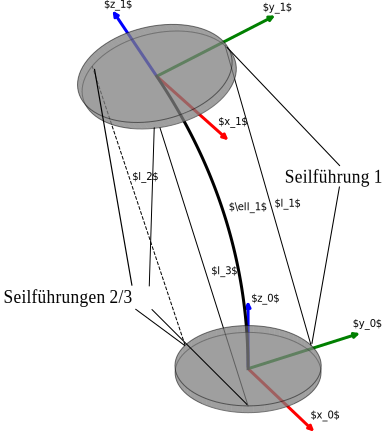
\includegraphics[width=.48\linewidth]{bilder/standdertechnik/continuum_robot3d.pdf}}
\begin{figure}[htb!]
\begin{subfigure}[t]{0.48\textwidth}
% füge bild ein, indem im Verhältnis zur definierten Box das Bild verschoben wird
\centering\raisebox{\dimexpr.5\ht\imagebox-.5\height}{
	\def\svgwidth{\textwidth}
	\input{bilder/standdertechnik/base.pdf_tex}
}
\caption{Trennscheibe der Roboterbasis}
\end{subfigure}
\begin{subfigure}[t]{0.48\textwidth}
\centering
\def\svgwidth{\textwidth}
\input{bilder/standdertechnik/continuum_robot3d.pdf_tex}
\caption{Segment des seilzugaktuierten kontinuierlichen Manipulators mit zwei Trennscheiben}
\end{subfigure}
\caption[Exemplarische Darstellung der Formgebung durch Seilzüge]{Exemplarische Darstellung der Formgebung durch Seilzüge}
\label{fig:roboterDesign}
\end{figure}

Die Krümmung des Kontinuumsroboters, bedingt durch die Seillängen und den Abstand der Seilführungen zum zentralen Rückgrat $d$, lautet
\begin{align}
\kappa = 2\frac{\sqrt{l_1^2+l_2^2+l_3^2-l_1l_2-l_2l_3-l_1l_3}}{d(l_1+l_2+l_3)}.
\label{eq:kappa}
\end{align}

Der Rotationswinkel des Kontinuumsroboters aus der $x$-$z$-Ebene wird durch
\begin{align}
\phi = \tan^{-1}\left(\frac{\sqrt{3}}{3} \frac{l_3+l_2-2l_1}{l_2-l_3} \right)
\label{eq:phi}
\end{align}

ermittelt. Für die numerische Berechnung des Rotationswinkels wurde die Erweiterung der inversen Tangensfunktion $atan2(x, y)$, die die Vorzeichen der beiden Funktionsargumente $x$ und $y$ berücksichtigt, verwendet. Dadurch lässt sich der Rotationswinkel auf den Wertebereich von $[0~2\pi]$ abbilden. Zuletzt wird die Segmentlänge 
\begin{align}
\ell = \dfrac{nd(l_1+l_2+l_3)}{\sqrt{l_1^2+l_2^2+l_3^2-l_1l_2-l_2l_3-l_1l_3}} 
\sin^{-1}\left( \frac{\sqrt{l_1^2+l_2^2+l_3^2-l_1l_2-l_2l_3-l_1l_3}}{3nd} \right)
\label{eq:ell}
\end{align}

bestimmt. Die Anzahl der Trennscheiben beträgt $n$. Zwischen zwei Treinnscheiben wird angenommen, dass die Seilzüge eine Krümmung aufweisen. Erhöht man die Anzahl der Führungsscheiben theoretisch mit~$\lim n\to \infty$ entspricht dies einer Formgebung des kontinuierlichen Manipulators mit sich kontinuierlich krümmenden Aktoren~\cite{JW06}. Der Fall $l_1=l_2=l_3$ entspricht der singulären Stellung mit $\kappa = 0$, welcher für die Transformationsmatrix im vorigen Abschnitt bereits behandelt wurde. Für den Nennerterm des ersten Faktors von~\eqref{eq:ell} folgt $\sqrt{l_1^2+l_2^2+l_3^2-l_1l_2-l_2l_3-l_1l_3} = 0$. Damit wäre die Berechnung der Segmentlänge im singulären Fall anhand~\eqref{eq:ell} nicht möglich. Im ausgesteckten Zustand des Roboters entspricht die Segmentlänge der Länge der Seilzüge \mbox{$\ell= (l_1+l_2+l_3)/3$}.


Für die roboterspezifische Kinematik ist eine konstante Segmentlänge eine häufig gestellte Annahme. Dadurch lassen sich nur zwei Seillängen pro Segment unabhängig voneinander einstellen. Die dritte ist durch die Zwangsbedingung der konstanten Segmentlänge vorbestimmt. 
Im Rahmen dieser Arbeit weist die Kinematik eine variable Segmentlänge auf. Dadurch ist jedes einzelne Segment ein- und ausfahrbar. Die roboterspezifische Kinematik richtet sich damit maßgeblich nach~\cite{JW06a}. In der angegebenen Veröffentlichung wird die Kinematik eines aus mehreren Segementen und seilzugaktuierten Kontinuumsroboters behandelt. Insbesondere werden für die Gelenkwinkel Aktorgrenzen berücksichtigt, die nicht durch eine konstante Segmentlänge eingeschränkt sind. Die stellbaren \mbox{Gelenkwinkel $l_1, l_2, l_3$} werden durch eine untere und obere Grenze $l_{\mathrm{min}}$ bzw. $l_{\mathrm{max}}$ beschränkt. Seilzüge können prinzipiell nur Zugkräfte aufbauen und wären somit nicht in der Lage, den kontinuierlichen Manipulator über Aufbringen von Druckkräften zu strecken. Eine Realisierung von Druckkräften ist prinzipiell mit einer an dem Rückgrat angebrachten Federvorrichtung möglich. Diese wird in Abhängigkeit von den eingestellten Gelenkwinkeln gestaucht oder gestreckt. Außerdem können die Seilzüge antagonistisch angeordnet werden, um Druckkräfte aufzubauen. Die Möglichkeiten, Druckkräfte zu entwickeln, werden an dieser Stelle nur erwähnt, aber im Weiteren nicht weiter berücksichtigt. \newline

Mit~\eqref{eq:kappa},~\eqref{eq:phi},~\eqref{eq:ell} wird an dieser Stelle die vektorwertige Funktion
\begin{align}
\bm{f}_{\mathrm{s}} =
\begin{bmatrix}
\kappa \\ \phi \\ \ell
\end{bmatrix} = 
\begin{bmatrix}
2\frac{\sqrt{l_1^2+l_2^2+l_3^2-l_1l_2-l_2l_3-l_1l_3}}{d(l_1+l_2+l_3)} \\
\tan^{-1}\left(\frac{\sqrt{3}}{3} \frac{l_3+l_2-2l_1}{l_2-l_3} \right) \\
\dfrac{nd(l_1+l_2+l_3)}{\sqrt{l_1^2+l_2^2+l_3^2-l_1l_2-l_2l_3-l_1l_3}} 
\sin^{-1}\left( \frac{\sqrt{l_1^2+l_2^2+l_3^2-l_1l_2-l_2l_3-l_1l_3}}{3nd} \right)
\end{bmatrix}
\label{eq:fSpezifischVektor}
\end{align}

der Vollständigkeit halber angegeben. \newline

Mit den Ergebnissen der letzten beiden Abschnitte kann die gesamte, direkte kinematische Kette  
\begin{align}
\bm{x}_\mathrm{E} = \bm{f}_\mathrm{u} \left( \bm{f}_\mathrm{s} \left( [l_1, l_2, l_3]^\transpose \right) \right)
\label{eq:kinematischeKette}
\end{align}

eines seilzugaktuierten Kontinuumsroboters für ein Segment gebildet werden. Die Kinematik für mehrere Verknüpfte Segmente eines Kontinuumsroboters ist Gegenstand des nächsten Abschnitts.

\subsection{Vorwärtskinematik mehrerer Segmente eines Kontinuumsroboters}
\label{subsec:multikinematik}

In den letzten beiden Abschnitten wurde der Grundstein für die direkte Kinematik eines seilzugaktuierten Kontinuumsroboter gelegt. Die Ergebnisse werden genutzt, um die Vorwärtskinematik eines kontinuierlichen Manipulators mit mehreren verknüpften Segmente zu ermitteln. \newline

Mit einer Verkettung von insgesamt $j$ homogenen Transformationsmatrizen
\begin{align}
{}^{0}\bm{T}_j = {}^{0}\bm{T}_{1} {}^1\bm{T}_{2} \dots {}^{j-1}\bm{T}_{j}
\end{align}

lässt sich die eine beliebige Lage entlang von $j$ Segmenten transformieren. In dieser Arbeit werden lediglich zwei Segmente modelliert. Es folgt ${}^{0}\bm{T}_2 = {}^{0}\bm{T}_{1} {}^1\bm{T}_{2}$ mit sechs Gelenkwinkeln~$\bm{q} = \left[l_{1,1}, l_{1,2}, l_{1,3}, l_{2,1}, l_{2,2}, l_{2,3} \right]^\transpose$. 
Der erste Index der Seillängen bestimmt das Segment, an dem der Seilzug endet. Der Segmentindex steigt, beginnend bei der Roboterbasis, auf. Der zweite Index legt den Seilzug gemäß Bild~\ref{fig:roboterDesign} fest. Die effektiven Seillängen des zweiten Segments, die für die Berechnung der roboterspezfischen Kinematik benötigt werden, lauten:
\begin{align}
l_{2,i,\mathrm{e}} = l_{2,i} - l_{1,i}\text{\,}, \text{für~} i = 1,2,3.
\label{eq:effektiveLaenge}
\end{align}

Die Seilzüge beider Segmente verlaufen jeweils durch dieselben Seilführungen der Trennscheiben. Es wird angenommen, dass die Seilzüge der jeweiligen Segmente die Formgebung des anderen Segments nicht beeinflussen. Dies stellt eine starke Vereinfachung dar, welche im Allgemeinen nicht gültig ist~\cite{WIJ10}. Diese Vereinfachung wird jedoch in Kauf genommen, da das Erlernen der inversen Kinematik im Vordergrund steht und nicht eine möglichst realistische Gestaltung der Kinematik beabsichtigt wird. \newline

Damit ist die Vorwärtskinematik für einen seilzugaktuierten Kontinuumsroboter mit zwei Segmenten vollständig beschrieben. Die Inverskinematik wird im folgenden Abschnitt behandelt.


\subsection{Inverse Kinematik}
\label{subesc:inverseKinematik}

Für serielle Roboter sowie auch Kontinuumsroboter gestaltet sich die Ermittlung der inversen Kinematik im Allgemeinen komplizierter als die der direkten. Zwei bestehende Konzepte zur Berechnung der inversen Kinematik eines kontinuierlichen Manipulators werden in diesem Abschnitt vorgestellt. Als erstes wird eine geometrische Ermittlung erläutert. Im Anschluss wird die differentielle Inverskinematik über die Berechnung von Jacobimatrizen vorgestellt. \newline

Ordnet man einer gegebenen Endeffektorlage eine Gelenkwinkelkonfiguration zu, spricht man von der Invers- bzw. inversen Kinematik
\begin{align}
\bm{q}  = \bm{f}^{-1} \left( \bm{x}_{\mathrm{E}} \right), 
\label{eq:inverskinematik}
\end{align} 

wobei $\bm{f}^{-1}$ die inverse Funktion zu $\bm{f}$ darstellt. In Hinblick auf Kontinuumsroboter mit stückweise konstanter Krümmung lässt sich die Inverskinematik in einen roboterunabhängigen Teil
\begin{align}
\left[ \kappa, \phi, \ell \right]^\transpose = \bm{f}^{-1}_{\mathrm{u}} \left( \bm{x}_{\mathrm{E}} \right)
\end{align}

und einen roboterspezfischen Teil
\begin{align}
\bm{q} = \bm{f}^{-1}_{\mathrm{s}} \left( \kappa, \phi, \ell \right)
\end{align}

aufteilen. Damit sind alle in Bild~\ref{fig:kinematikraeume} aufgeführten kinematischen Komponenten definiert. \newline

Zunächst wird die geometrische Lösung der inversen Kinematik erläutert.
Die inverse, roboterspezifische Funktion eines seilzugaktuierten Manipulators ist in~\cite{JW06} gegeben. Die Seillängen für ein Segment lassen sich geometrisch in Abhängigkeit der Kreisbogenparameter wie folgt berechnen:
\begin{align}
\bm{f}^{-1}_{\mathrm{s}} \left( \kappa, \phi, \ell \right) = 
\begin{bmatrix}
l_1 \\ 
l_2 \\
l_3 
\end{bmatrix}
=
\begin{bmatrix}
2n \sin \left( \dfrac{\kappa c}{2n} \right) \left( \dfrac{1}{\kappa} - d \sin\phi \right) \\
2n \sin \left( \dfrac{\kappa c}{2n} \right) \left( \dfrac{1}{\kappa} + d \sin \left(\dfrac{\pi}{3} + \phi  \right) \right) \\
2n \sin \left( \dfrac{\kappa c}{2n} \right) \left( \dfrac{1}{\kappa} - d \cos \left(\dfrac{\pi}{6} + \phi  \right) \right) \\
\end{bmatrix}
\label{eq:fInversSpezifisch}
\end{align}

Damit ist prinzipiell nur noch die Bestimmung der inversen, roboterunabhängigen Kinematik notwendig. Es sind resultierende Kreisbogenparameter aus einer gegebenen Endeffektorlage gesucht. Neppalli et al. beschreiben in~\cite{NCJW09} ein Verfahren zur geometrischen Ermittlung von Kreisbogenparamtern $\kappa, \phi, \ell$ aus einer gegebenen Endeffektorposition für einen Kontinuumsroboter mit $j$ Segmenten. Die Autoren lösen das beschriebene Problem mittels mehrerer Algorithmen, die in Tabelle~\ref{tab:geometrischeInverseUnabhaengigeKinematik} mit ihren Ein- und Ausgangsgrößen zusammengefasst sind. Die gewonnenen Bogenparameter können mit~\eqref{eq:fInversSpezifisch} in Seillängen des Kontinuumsroboters umgerechnet werden. 

Ein Nachteil der vorgestellten geometrischen Bestimmung von Bogenparametern besteht darin, dass die Abstände zwischen den Endpositionen der Robotersegmente vorgegeben werden müssen, siehe~\ref{tab:geometrischeInverseUnabhaengigeKinematik}\,(a). Desweitern berücksichtigt dieser Ansatz keine Aktorgrenzen. Zuletzt ist die Orientierung des Endeffektors nicht Teil der Kinematik. \newline

\begin{table}[htb!]
\caption[Generelles Vorgehen der geometrischen Bestimmung von Kreisbogenparametern]
{Generelles Vorgehen der geometrischen Bestimmung von Kreisbogenparametern anhand einer gegeben Endeffektorlage nach~\cite{NCJW09}}
\begin{tabular}{ l  p{7.5cm} | p{6.50cm}}
\label{tab:geometrischeInverseUnabhaengigeKinematik}	
& \multicolumn{1}{c}{Eingangsgrößen} & \multicolumn{1}{c}{Ausgangsgrößen}\\ \hline\hline
(a) & Endeffektorposition $\bm{x}_{\mathrm{E,p}} = \bm{x}_{j,\mathrm{p}}$, Abstände zwischen den Endpositionen der einzelnen Robotersegmente \mbox{$d_i = ||\bm{x}_{i,\mathrm{p}}-\bm{x}_{i\shortminus1,\mathrm{p}}||_2$,} \mbox{$i = 1, \dots j $}, mit $\bm{x}_{0,\mathrm{p}} = \bm{0}$ & Endpositionen $\bm{x}_{i,\mathrm{p}}$, $i = 1,\dots j \shortminus 1$ \\ \hline
(b) & Endpositionen $\bm{x}_{i,\mathrm{p}}$, $i = 1, \dots j$, welche in die Roboterbasis transformiert werden &  Bogenparameter $\kappa_i, \phi_i, \ell_i$, $i \shortequal 1,  \dots j$ unter Anwendung von (c)  \\ \hline
(c) & Beliebige Position $\bm{x}_{\mathrm{p}}$ &  Bogenparameter $\kappa, \phi, \ell$ in Bezug zur Roboterbasis \\ 
\end{tabular}
\end{table}

Der nächste Ansatz löst die differentielle Kinematik
\begin{align}
\dot{\bm{x}}_{\mathrm{E}} = \bm{J} \mkern-1mu( \bm{q} ) \bm{q}
\label{eq:differentielleKinematik}
\end{align}

mit der Jacobi-Matrix $\bm{J}\mkern-1mu (\bm{q})$. Über eine Invertierung der Jacobi-Matrix lässt sich die inverse, differentielle Kinematik 
\begin{align}
\dot{\bm{q}} = \bm{J}^{-1} \mkern-1mu( \bm{q} ) \dot{\bm{q}}
\label{eq:differentielleInverseKinematik}
\end{align}

ermitteln. Nach~\cite{JW06} wird die folgende kinematischen Kette
\begin{align}
\bm{x}_{\mathrm{E}} 
\stackrel{\bm{f}_{\mathrm{DH}}}{\parbox{1cm}{\leftarrowfill}} \bm{\theta}, \bm{d}
\stackrel{\bm{f}_1}{\parbox{1cm}{\leftarrowfill}} \kappa, \phi, c
\stackrel{\bm{f}_2}{\parbox{1cm}{\leftarrowfill}} \bm{l}
\label{eq:informationsflussJonesWalker}
\end{align}

aufgestellt. Die vektorwertige Funktion $\bm{f}_2$ entspricht dabei der bereits aufgeführten roboterspezifischen Kinematik gemäß~\eqref{eq:fSpezifischVektor}, welche die Seillängen~$\bm{l}$ in Bogenparameter übersetzt. Mithilfe der gewonnenen Bogenparameter werden zunächst klassische \textit{Denavit-Hartenberg}-Parameter~$\bm{\theta, \bm{d}}$ mittels $\bm{f}_1$ aufgestellt. Diese können widerrum mit~$\bm{f}_{\mathrm{DH}}$ zur Bishop-Transformationsmatrix, gegeben durch~\eqref{eq:T_bishop}, überführt werden. Dadurch unterscheidet sich das Vorgehen von der Bestimmung der direkten, roboterunabhängigen Kinematik in Abschnitt~\ref{subsec:unabhaengigeVorwaertskinematik}, bei der die Transformationsmatrix direkt aus Bogenparametern ermittelt wird. Aus den einzelnen kinematischen Komponenten ermitteln die Autoren über eine Verkettung der Jacobi-Matrizen
\begin{align}
\dot{\bm{x}}_{\bm{\mathrm{E}}} = \bm{J}_{\mathrm{DH}} \bm{J}_{\bm{f}_1} \bm{J}_{\bm{f}_2}  \dot{\bm{l}} 
= \bm{J}\mkern-1mu (\bm{l}) \dot{\bm{l}}
\label{eq:modulareDifferentielleKinematik}
\end{align}

die differentielle Kinematik. Der modulare Aufbau der differentiellen Kinematik erlaubt es, diverse Hardware-Designs, die lediglich eine Anpassung der spezifischen Funktion $\bm{f}_2$ benötigen, zu realisieren. Außerdem ist eine echtzeitfähige Steuerung der Kinematik mit
\begin{align}
\dot{\bm{l}} = \bm{J}^{+} \mkern-2mu(\bm{l}) \dot{\bm{x}}
\label{eq:inverseDifferentielleKinematik}
\end{align}

möglich. Es ist $\bm{J}^{+}$ die Pseudoinverse zu $\bm{J}$, eine Verallgemeinerung der inversen Matrix auf singuläre und nichtquadratische Matrizen. \newline

Es wurden zwei Wege aufgezeigt, mit denen die inverse Kinematik eines seilzugaktuierten, kontinuierlichen Manipulators umgesetzt werden kann. Die Grundbausteine des Reinforcement-Learnings werden nachstehend dargelegt, bevor die in diesem Werk erarbeitete Methode der Inverskinematik von existierenden Ansätzen abgegegrenzt wird.

%Zuletzt wird die Ermittlung der inversen Kinematik nach~\cite{TFCL16} beschrieben. In der Veröffentlichung wird 

\section{Bestärkendes Lernen im Kontext des maschinellen Lernens}
\label{sec:RLallgemein}

Die Notation von Größen des Reinforcement Learning richtet sich größtenteils nach dem von Sutton und Barto verfasstem Standardwerk~\cite{SB98} für Reinforcement Learning. 




\begin{enumerate}
\item \textbf{Kontinuumsrobotik}
\begin{enumerate}

\item Kurz Unterschiede der Freiheitsgrade zwischen seriellen und kontinuierlichen Strukturen. Redundant $\rightarrow$ hyperredundant $\rightarrow$ kontinuierlich

\item Kontinuumsroboter Randphänomen in der industriellen Robotik, wo serielle Roboter die Domäne dominieren aufgrund ihrer Genauigkeit und Präzision. Spezialisierung auf bestimmte Bewegungen mit bestimmten Manipulatoren. Ein Großteil der seriellen Roboter versucht den Menschen oder Tiere zu imitieren (Arme, humanoide)

\item konzentrisch Rohre haben gute Anwendungsgebiete in der minimalinvasiven Chirurgie

\item Derzeitige Forschungsgebiete/Anwendungsgebiete: Metabot (https://www.lkr.uni-hannover.de/projects.html)

\item Parallelkontinuierliche Manipulatoren (PCR), die vorher nur mit seriellen Gliedern erforscht und produziert wurden.

\item Medusa (https://www.lkr.uni-hannover.de/medusa.html)

\item Anwendung in der Medizintechnik.

\item Aufzeigen des in dieser Arbeit verwendeten Kontinuumsroboter.

\end{enumerate}
\item \textbf{Kinematik von kontinuierlichen Manipulatoren}
\begin{enumerate}

\item Zum Thema Genauigkeit der Kinematik ist zu sagen: kontinuierliche Manipulatoren können grundsätzlich nicht so genau kinematische modelliert werden, wie serielle Roboter mit rigiden Strukturen. Die inhärente Steifigkeit erlaubt es hohe Wiederhol- und Positioniergenauigkeiten zu realisieren. Die Nachgiebigkeit der Kontinuumsroboter führt zu größeren Fehlern in diesem Zusammenhang, bzw. Abweichung der erwarten kalkulierten kinematischen Genauigkeit. Der Einfluss von äußeren Quellen wie Gravitation oder Beladung des Endeffeketors oder umgriffener Gegenstand verändert die nachgiebige Struktur des Roboters zusätzlich. Dieser Einfluss wird zunächst in vielen kinematischen Modellen vernachlässigt. Jedoch kann gerade diese Nachgiebigkeit in schwer zugänglichen Räumen genutzt werden um sich zum Beispiel in einen Pfad zu winden. Aber das ist gerade nicht so schlimm, weil die Nachgiebigkeit in vielen Fällen erwünscht ist. Zum Beispiel beim Umgreifen eines Gegenstands soll sich der kontinuierliche Manipulator an das Objekt anschmiegen. Oder bei der Verwendung eines Geräts für Hals soll sich das Gerät der Halsform anpassen. 

\end{enumerate}
\item \textbf{Maschinelles Lernen und im Speziellen \textit{Reinforcement Learning}}
\begin{enumerate}
\item huhu
\end{enumerate}

\end{enumerate}

\begin{itemize}

\item Direkte Kinematik bereits etablierte Modelle für konstante Krümmungen. Es wird das kinematische Modell aus "Kinematics for Multisection Continuum Robots" verwendet. Es liefert eine geometrische Zusammenhänge zwischen der Aktuierung der Seilzüge und der daraus resultierende Krümmung des kontinuierlichen Manipulators.

\item Seilzugaktuierte können entweder über kompressibel Federn gestützt oder über antagonistische Seilzüge bedient werden. Inkompressibles Design ist populär. In dieser Arbeit wird aber kompressibel Design gewählt.

\item ??Darstellung von Orientierungen, Euler-Winkel, Achse-Winkel, Quaternionen. Abgrenzung Vorteile Quaternionen sollten immer verwendet werden??

\item Darstellung verschiedener Ansätze zur inversen Kinematik. 

\item Geometrische Lösung der inversen Kinematik mittels Zwischenpunkten jedes Segments (A Geometrical Approach to Inverse Kinematics for Continuum Manipulators, Neppalli et al.) \cite{NCJW09}

\item Geometrische Inverse Kinematik: Aber benötigt Endpunkte aller Segmente

\item Abgrenzung zu meinem Ansatz. Simulative Lösung die sowohl ohne Orientierung nud mit Berücksichtigung der Orientierung löst. 

\item Inverse Kinematik mittels Supervised Learning

\item Mein Ansatz mittels Reinforcement Learning

\item Darauf aufmerksam machen, dass man beim Reinforcement learning ansatz einen bisher nicht erforschten Weg gefunden hat. --> Recherche nach Papern. 

\item RL als Gruppe von Methoden des maschinellen Lernens (Supervised, Unsupervised, RL) darstellen. 

\item in RL geht es darum abhängig vom derzeitigen Zustand Entscheidungen zu treffen. Getroffene Entscheidungen werden meistens von einem Agent Aktionen ausgeführt.

\item Ausgangspunkt des RL ist oft der sogenannte Markow-Entscheidungsprozess. 

\item RL Methoden, vor allem Deep RL und das neuronale Netz

\item Die Bedeutung von künstlichen neuronalen Netzen im Reinforcement Learning beschreiben

\item Verwendung von künstlichen neuronalen Netzen für Funktionsapproximierung - Skalierung des RL auf hochdimensionale Anwendungsgebiete

\item RL Errungenschaften - Heli, GO, Dota2/OpenAiFive

\item RL in der Realität: Problematik curse of dimensionality, und Datengenerierung - Zurücksetzen des Ausgangszustands. Beispiel google mit roboterfarm die greifen (https://ai.googleblog.com/2018/06/scalable-deep-reinforcement-learning.html)

\end{itemize}




